\subsection{Operación Básica con Punto Fijo}

Para esta sección se considera el caso de aplicar un enventanamiento con una ventana Blackman a un vector de $N=161$ datos de audio. Se supone que se debe operar usando aritmética de punto fijo y que el ADC entrega las muestras cuantizadas como un número entero con signo \texttt{int16}.

\begin{enumerate}[a)]
    \item Se lee el archivo \texttt{aliasing\_test\_16\_16.wav} con su tipo de dato nativo (\texttt{int16}) y se rescatan en la variable $x$ las primeras $N$ muestras.
    
    Notar que al utilizar \texttt{audioread(aliasing\_test\_16\_16.wav)} para leer el archivo de audio se obtiene un vector de datos tipo \texttt{double} de máxima amplitud igual a 1. Comparando con la máxima amplitud de los datos obtenidos al leer el archivo en formato nativo se concluye que el vector de datos corresponde a la representación interna utilizando 16 bits en $Q15$.
    
    \begin{figure}[H]
        \centering
        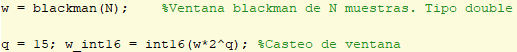
\includegraphics{imagenes2/p6_blackman.png}
        \caption{Código en MATLAB para obtener una ventana Blackman como un vector de datos de 16 bits en $Q15$.}
        \label{fig:p6_blackman}
    \end{figure}
    
    La sección de código para obtener la ventana Blackman como un vector de datos de 16 bits en $Q15$ se muestra en la figura \ref{fig:p6_blackman}. Del código puede comentarse que:
    \begin{itemize}
        \item En la primera línea se obtiene una ventna blackman de $N$ datos, los cuales son de tipo \texttt{double}.
        \item La segunda línea corresponde a la transformación a formato 16 bits $Q15$. Recordar que:
        $$ w = w_{ri}\cdot 2^{-q}$$
        donde $w$ representa la ventana, $w_{ri}$ la ventana en representación interna y $q$ el número de bits que correspoden a decimales.
        
        Como se dispone de la ventana en formato \texttt{double}, se debe despejar $w_{ri}$ para obtener la ventana en 16 bits $Q15$, que es precisamente lo que se hace en la segunda línea. 
    \end{itemize}
    
    Aplicando el comando \texttt{whos} se obtiene que:
    \begin{itemize}
        \item La ventana con datos de tipo \texttt{double} ocupa 1288 bytes.
        \item La ventana con datos de tipo \texttt{int16} ocupa 322 bytes.
    \end{itemize}
    
    Como era de esperarse, se ocupa 4 veces menos memoria, lo cual resulta una mejora considerable asumiendo que se cuenta con hardware para operación en punto fijo.
    
    Posteriormente se aplica el enventanamiento en punto fijo.
    
    \begin{figure}[H]
        \centering
        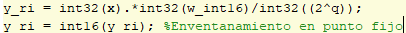
\includegraphics{imagenes2/p6_pond.png}
        \caption{Código en MATLAB para obtener enventanamiento simulando operación en punto fijo.}
        \label{fig:p6_pond}
    \end{figure}
    
    La sección de código para obtener la ventana Blackman como un vector de datos de 16 bits en $Q15$ se muestra en la figura \ref{fig:p6_blackman}. Del código puede comentarse que:
    
    \begin{itemize}
        \item La primera y segunda línea corresponden a la obtención del producto en representación interna. Recordar que
        $$ c = a\cdot b = (a_{ri}\cdot b_{ri}\cdot 2^{-q})\cdot 2^{-q}\Rightarrow c_{ri} = a_{ri}\cdot b_{ri}\cdot 2^{-q}$$
        donde el $ri$ hace referencia a la representación interna en $Qq$, siendo $q$ el número de bits correspondientes a decimales.
        
        Con lo anterior resulta claro que la primera línea corresponde a la obtención en representación interna de $y$, donde se trabaja con datos \texttt{int32} por el overflow de la multiplicación. En la segunda se vuelve al tipo de dato \texttt{int16}. 
    \end{itemize}
    
    Aplicando el comando \texttt{whos} se obtiene que:
    \begin{itemize}
        \item El enventanamiento (ponderación) con datos de tipo \texttt{double} ocupa 1288 bytes.
        \item El enventanamiento (ponderación) con datos de tipo \texttt{int16} ocupa 322 bytes.
    \end{itemize}
    
    obteniendo nuevamente un factor de 4 veces menos memoria al operar con datos \texttt{int16}. 
    
    Finalmente se obtiene una representación gráfica de la señal $x$, $w$ e $y$ en representación interna, la cual aparece en la figura \ref{fig:p6_graf}. Visualmente se aprecia la ponderación es correcta.
    
    \begin{figure}[H]
        \centering
        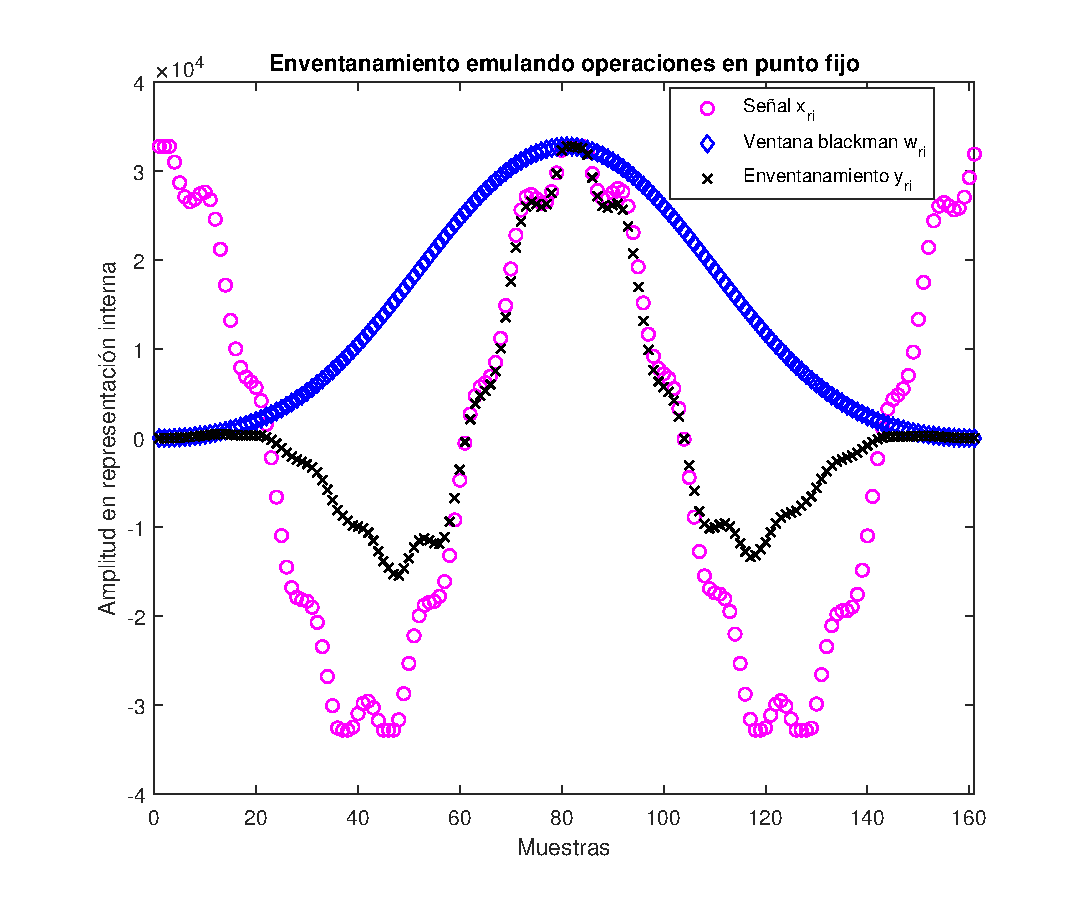
\includegraphics[width = .9\linewidth]{imagenes2/p6_graf.eps}
        \caption{Señales $x$, $w$ e $y$ en representación interna vs muestras.}
        \label{fig:p6_graf}
    \end{figure}
    
\end{enumerate}